\subsection{Obstacle avoidance : exploration with left and right recursive search}

When the robot wants to move to a specific position, he first checks if any other robot is in his way (direct line between him and the target), if there is it initiates a pathfinding algorithm to explore alternative routes. This exploration phase involves adjusting the robot’s direction by incrementally rotating the vector facing the target, to the left and to the right, until a free angle is identified. The exploration tree is a binary tree with a branch going to the left and the other to the right of the robot.

\paragraph{Obstacle Detection and Rotation}

Upon detecting an obstacle, the robot begins exploring by rotating incrementally in one direction (e.g., left) (check figure \ref{fig:path_finding} to have a better understanding). After each small rotation, it evaluates whether the new direction results in a clear path of a short length. The robot checks if any obstacles intersect the trajectory.

Free Angle: If no obstacles block the path, the angle is marked as “free,” and the robot proceeds along this trajectory.

Obstacle Detected: If an obstacle remains, the robot continues rotating further in the same direction (left or right) until a free path is found or the maximum angle limit is reached.

\paragraph{Recursive Exploration}

When a free path is identified, the algorithm recursively evaluates the next step from the new position. It continues checking whether this position brings the robot closer to the target while considering any new obstacles in its way. The exploration process repeats until the target is reached or the maximum itteration number is reached.

\paragraph{Trajectory Smoothing}

Once a path is calculated, it is smoothed to eliminate unnecessary waypoints, retaining only significant points to optimize the trajectory.

\paragraph{Optimal Direction Selection}

If both left and right explorations yield free paths, the algorithm selects the optimal path based on proximity to the target. If no fully clear path is found, the robot moves along the trajectory that gets it closest to the target.

\paragraph{Continuous Recalculation}

The algorithm runs continuously, recalculating the best trajectory in real-time, ensuring dynamic responsiveness to changing environments.

\begin{figure}
    \centering
    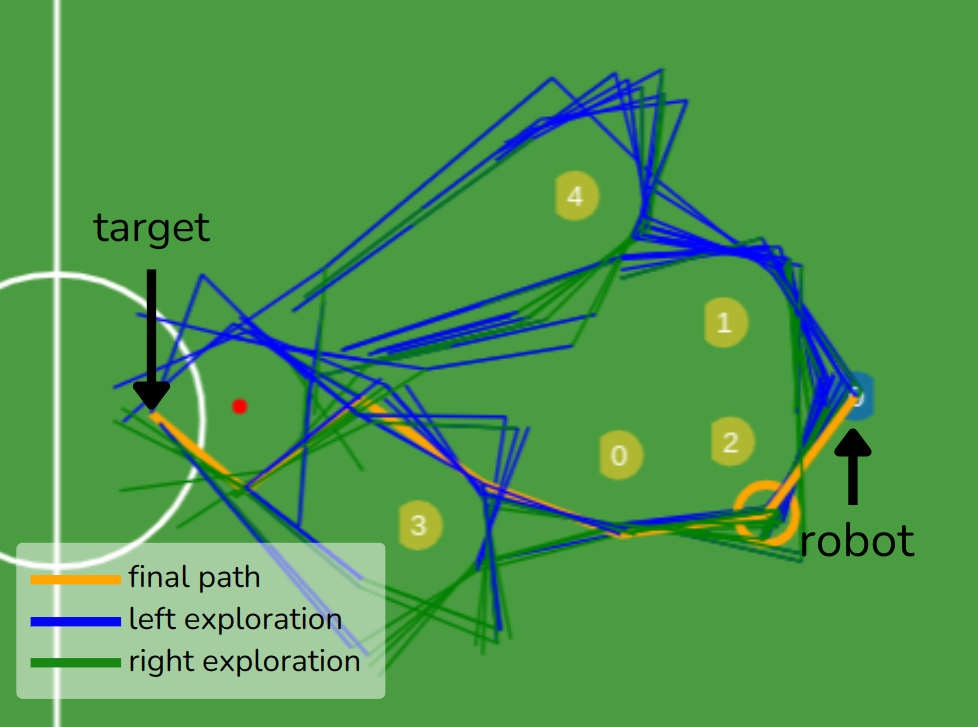
\includegraphics[scale=0.3]{path_finding.png}
    \caption{Path finding example}
    \label{fig:path_finding}
\end{figure}
